\documentclass[@BEAMER_OPTIONS@]{beamer}
    @USE_PGFPAGES@

    \usetheme[alternativetitlepage=true,titleline=true]{Torino}
    \setbeamertemplate{navigation symbols}{}
    \setbeamertemplate{note page}[plain]
    \setbeamertemplate{caption}{\insertcaption}

    \usepackage[utf8]{inputenc}
    \usepackage[russian]{babel}
    \usepackage{graphicx}
    \usepackage{subfigure}
    \usepackage{xspace}
    \usepackage{adjustbox}
    \usepackage{tikz}
    \usepackage{relsize}
    \usepackage{fancyvrb}
    \fvset{fontsize=\footnotesize}
    \RecustomVerbatimEnvironment{verbatim}{Verbatim}{}
    \usepgflibrary{arrows}
    \usetikzlibrary{shadows,decorations.pathreplacing,patterns,shapes}
    \tikzstyle{every picture}=[semithick,>=stealth,remember picture]
    \usepackage{listings}
    \lstset{
        language=C++,
        basicstyle=\footnotesize\rmfamily,
        stringstyle=\color{chameleon3},
        numbers=left,
        numberstyle=\tiny,
        aboveskip=-0.02\baselineskip,
        belowskip=-0.02\baselineskip,
        columns=flexible,
        extendedchars=false,
        showstringspaces=false,
        morekeywords={global,kernel,ulong,size_t,get_global_id,get_global_size}
        }
    \newcommand{\code}[1]{\lstinline|#1|}
    \newcommand{\additive}{\hspace{1cm}\footnotesize(\emph{Additive expressions only})}
    \newcommand{\singledevice}{\hspace{1cm}\footnotesize(\emph{Single-device contexts})}
    \protected\def\plusplus{{\nolinebreak[4]\hspace{-.05em}\raisebox{.4ex}{\relsize{-3}\bf ++}}\xspace}
    \newcommand{\CXX}{{\rm C}\plusplus}
    \newcommand{\CC}{{\rm C99}\xspace}
    \newcommand{\ghribbon}{
        \begin{tikzpicture}[remember picture,overlay]
            \node[anchor=north east,yshift=4pt,xshift=4pt] at (current page.north east) {
                \href{https://github.com/ddemidov/vexcl}{
\includegraphics[width=2cm]{forkme}}
            };
        \end{tikzpicture}
    }

    \title{VexCL}
    \subtitle{Генерация ядер OpenCL/CUDA из выражений \CXX}

    \author{Денис Демидов}
    \institute{ МСЦ РАН, Казань \\ \vspace{\baselineskip} }
    \date{Октябрь 2014, Таруса}

\begin{document}

%----------------------------------------------------------------------------
\begin{frame}{}
    \titlepage
\end{frame}

\note{ }

%----------------------------------------------------------------------------
\section{Введение}
\begin{frame}{Современные GPGPU платформы}
    \begin{columns}
        \begin{column}{0.45\textwidth}
            \begin{block}{NVIDIA CUDA}
                \begin{itemize}
                    \item Проприетарная архитектура
                    \item Необходимо аппаратное обеспечение NVIDIA
                    \item Зрелое окружение, большое число библиотек
                        \vspace{\baselineskip}
                    \item<2> \emph{Ядра (\CXX) компилируются в псевдо-ассемблер
                        (PTX) вместе с основной программой}
                \end{itemize}
            \end{block}
        \end{column}
        \begin{column}{0.45\textwidth}
            \begin{block}{OpenCL}
                \begin{itemize}
                    \item Открытый стандарт
                    \item Большой диапазон поддерживаемого железа
                    \item Низкоуровневый программный интерфейс
                        \vspace{\baselineskip}
                    \item<2> \emph{Ядра (\CC) компилируются во время
                        выполнения, увеличивается время инициализации}
                \end{itemize}
            \end{block}
        \end{column}
    \end{columns}
    \vspace{\baselineskip}
    \begin{itemize}
        \item<2> Последнее отличие обычно считается недостатком OpenCL.
        \item<2> Однако, это позволяет генерировать во время выполнения более
            эффективные ядра под конкретную задачу!
    \end{itemize}
\end{frame}

\note{ }

%----------------------------------------------------------------------------
\begin{frame}{VexCL}{Библиотека шаблонов векторных выражений для OpenCL/CUDA}
    \ghribbon
    \begin{itemize}
        \item Создана для облегчения разработки GPGPU приложений на \CXX.
            \begin{itemize}
                \item Интуитивная нотация для записи векторных выражений.
                \item Автоматическая генерация вычислительных ядер во время
                    выполнения.
            \end{itemize}
            \vspace{\baselineskip}
        \item Исходный код доступен под лицензией MIT.
            \begin{itemize}
                \item \href{https://github.com/ddemidov/vexcl}{https://github.com/ddemidov/vexcl}
            \end{itemize}
            \vspace{\baselineskip}
    \end{itemize}
\end{frame}

\note[itemize]{
\item VexCL is a vector expression template library for OpenCL. It uses
    template metaprogramming techniques (in particular, expression templates)
    to provide an intuitive notation for vector and matrix operations.
\item The source code of the library is available on GitHub. It is distributed
    under MIT license, so you are basically free to do whatever you want with
    the library.
\item I would like to note that this is not another C++ bindings library. VexCL
    is designed to work with standard C++ bindings for OpenCL that are provided
    by the Khronos group.
}

%----------------------------------------------------------------------------
\section{Программный интерфейс VexCL}
\begin{frame}
    \sectionpage
\end{frame}

\note{}

%----------------------------------------------------------------------------
\begin{frame}[fragile]{Пример использования VexCL: сложение векторов}
    \begin{exampleblock}{Инициализация конекста:}
        \begin{lstlisting}
vex::Context ctx( vex::Filter::DoublePrecision );
if ( !ctx ) throw std::runtime_error("No compute devices available");
        \end{lstlisting}
    \end{exampleblock}
    \begin{exampleblock}{Подготовка входных данных, перенос на GPU:}
        \begin{lstlisting}[firstnumber=last]
std::vector<double> a(N, 1), b(N, 2), c(N);
vex::vector<double> A(ctx, a);
vex::vector<double> B(ctx, b);
vex::vector<double> C(ctx, N);
        \end{lstlisting}
    \end{exampleblock}
    \begin{exampleblock}{Запуск вычислительного ядра, перенос результатов на CPU:}
        \begin{lstlisting}[firstnumber=last]
C = A + B;
vex::copy(C, c);
std::cout << c[42] << std::endl;
        \end{lstlisting}
    \end{exampleblock}
\end{frame}

\note[itemize]{
\item Here is the simplest example of using vexcl: addition of two vectors on a
    gpu card.
\item The first line is the context initialization. We provide a device filter
    to the context constructor and get all compute devices that satisfy the
    filter. Here we filter by type and get all available GPUs.
\item Data allocation and transfer is also simplified. \code{vex::vector}
    constructor allocates memory on device and possibly transfers initial data
    as well. The parameters here are list of command queues and either size or
    input host vector.
\item Line ten does what's needs to be done here. This simple expression leads
    to automatic kernel generation and launch. And then we copy the results
    back to host and see what we got.
}

%----------------------------------------------------------------------------
\begin{frame}[fragile]{Использование нескольких ускорителей}
    \setbeamercovered{transparent=40}
    \begin{exampleblock}{}
        \begin{onlyenv}<1|handout:0>
        \begin{lstlisting}[escapechar=!]
vex::Context ctx(
            vex::Filter::DoublePrecision && vex::Filter::Name("Tesla")
            );
        \end{lstlisting}
        \end{onlyenv}
        \begin{onlyenv}<2|handout:0>
        \begin{lstlisting}[escapechar=!]
vex::Context ctx(
            vex::Filter::DoublePrecision && vex::Filter::Type(CL_DEVICE_TYPE_GPU)
            );
        \end{lstlisting}
        \end{onlyenv}
        \begin{onlyenv}<3>
        \begin{lstlisting}[escapechar=!]
vex::Context ctx(
            vex::Filter::DoublePrecision
            );
        \end{lstlisting}
        \end{onlyenv}
        \begin{uncoverenv}<1>
        \begin{lstlisting}[firstnumber=last]

vex::vector<double> x(ctx, N);
vex::vector<double> y(ctx, N);

x = vex::element_index() * (1.0 / N);
y = sin(2 * x) + sqrt(1 - x * x);
        \end{lstlisting}
        \end{uncoverenv}
    \end{exampleblock}
    \setbeamercovered{invisible}
    \begin{figure}
        \begin{tikzpicture}
            \draw (0,2.5) rectangle +(8,0.1);
            \draw (0,2.5) grid[step=0.1] +(8,0.1);
            \draw (-0.3,2.6) node{x};

            \draw (0,2.0) rectangle +(8,0.1);
            \draw (0,2.0) grid[step=0.1] +(8,0.1);
            \draw (-0.3,2.1) node[anchor=center]{y};

            \uncover<1-3> {
            \draw (1,0.5) node{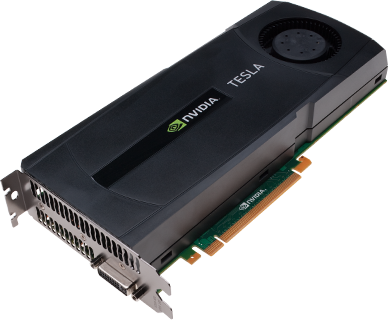
\includegraphics[width=0.2\textwidth]{tesla.png}};
            }

            \uncover<2-3> {
            \draw (4,0.5) node{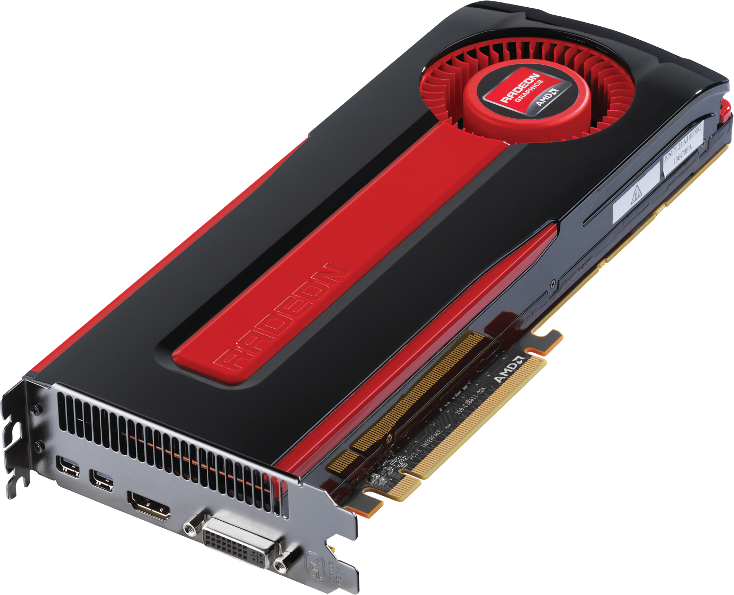
\includegraphics[width=0.2\textwidth]{radeon.png}};
            }

            \uncover<3> {
            \draw (7.5,0.5) node{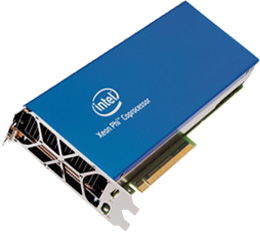
\includegraphics[width=0.17\textwidth]{intel.png}};
            }

            \uncover<1|handout:0> {
            \draw[->,chameleon2,style=dashed] (0,2.7) -- (0,1.8)
                .. controls +(east:0.5) and +(north west:0.5) ..
                (1.4,1.5);
            \draw[->,chameleon2,style=dashed] (8,2.7) -- (8,1.8)
                .. controls +(west:0.5) and +(north east:0.5) ..
                (1.6,1.5);
            }

            \uncover<2|handout:0> {
            \draw[->,chameleon2,style=dashed] (0,2.7) -- (0,1.8)
                .. controls +(east:0.5) and +(north west:0.5) ..
                (1.4,1.5);
            \draw[->,chameleon2,style=dashed] (4,2.7) -- (4,1.8)
                .. controls +(west:0.5) and +(north east:0.5) ..
                (1.6,1.5);

            \draw[->,chameleon2,style=dashed] (4,2.7) -- (4,1.8)
                .. controls +(east:0.1) and +(north west:0.2) ..
                (4.4,1.5);
            \draw[->,chameleon2,style=dashed] (8,2.7) -- (8,1.8)
                .. controls +(west:0.5) and +(north east:0.5) ..
                (4.6,1.5);
            }

            \uncover<3> {
            \draw[->,chameleon2,style=dashed] (0,2.7) -- (0,1.8)
                .. controls +(east:0.5) and +(north west:0.5) ..
                (1.4,1.5);
            \draw[->,chameleon2,style=dashed] (3,2.7) -- (3,1.8)
                .. controls +(west:0.5) and +(north east:0.5) ..
                (1.6,1.5);

            \draw[->,chameleon2,style=dashed] (3,2.7) -- (3,1.8)
                .. controls +(east:0.5) and +(north west:0.2) ..
                (4.4,1.5);
            \draw[->,chameleon2,style=dashed] (6,2.7) -- (6,1.8)
                .. controls +(west:0.5) and +(north east:0.5) ..
                (4.6,1.5);

            \draw[->,chameleon2,style=dashed] (6,2.7) -- (6,1.8) -- (7.4,1.5);
            \draw[->,chameleon2,style=dashed] (8,2.7) -- (8,1.8) -- (7.6,1.5);
            }
        \end{tikzpicture}
    \end{figure}
\end{frame}

\note[itemize]{
\item Now that we know how to initialize VexCL context, let's see how device
    vectors are allocated.
\item Here we allocate three vectors, and initialize two of them with
    constant values.
\item Each vector receives a list of queues at initialization.  Since each
    queue corresponds to a specific device, vectors know where to put their
    data to.
    \begin{enumerate}
        \item For example, if we only have the Tesla card in our context, then
            it will hold the complete memory for all of our vectors.
        \item If we use both of the available GPUs, then the vectors will be
            split between the devices. This split is by default proportional to
            the GPU bandwidth and is guaranteed to be consistent for vectors of
            the same size. This consistency allows VexCL to run computations
            independently on all devices in context.
        \item If we add the CPU to the context, it will get smaller share of
            the data and arithmetic operations.
    \end{enumerate}
\item Care must be taken with the use of several devices. VexCL tries to split
    the memory as fair as it can, but it is probable that your program will
    run at the speed of the slowest device.
}

%----------------------------------------------------------------------------
\begin{frame}[fragile]{Язык векторных выражений VexCL}
    \begin{itemize}
        \item Все векторы в выражении должны быть \emph{совместимыми}:
            \begin{itemize}
                \item Иметь один размер
                \item Быть расположенными на одних и тех же устройствах
            \end{itemize}
        \item Что можно использовать в выражениях:
            \begin{columns}
                \begin{column}{0.4\textwidth}
                    \begin{itemize}
                        \item Векторы, скаляры, константы
                        \item Арифм. и логич. операторы
                        \item Встроенные функции
                        \item Пользовательские функции
                        \item Генераторы случайных чисел
                        \item Сортировка, префиксные суммы
                    \end{itemize}
                \end{column}
                \begin{column}{0.4\textwidth}
                    \begin{itemize}
                        \item Временные значения
                        \item Срезы и перестановки
                        \item Редукция (сумма, экстремумы)
                        \item Произв. матрицы на вектор
                        \item Свертки
                        \item Быстрое преобразование Фурье
                    \end{itemize}
                \end{column}
            \end{columns}
    \end{itemize}
    \begin{exampleblock}{}
        \begin{lstlisting}
x = (2 * M_PI / n) * vex::element_index();
y = pow(sin(x), 2.0) + pow(cos(x), 2.0);
        \end{lstlisting}
    \end{exampleblock}
\end{frame}

\note[itemize]{
\item So, what kind of expressions can you use in VexCL?
\item First, any vectors used in an expression have to be compatible.
\item If this requirement is satisfied, then expressions may combine
    vectors and scalars with almost any binary operators. OpenCL math functions
    and user-defined functions are also available.
}

%----------------------------------------------------------------------------
\begin{frame}[fragile]{Ядра OpenCL/CUDA генерируются во время исполнения}
    \begin{columns}
        \begin{column}{0.33\textwidth}
            \begin{exampleblock}{Следующее выражение:}
                \begin{lstlisting}
x = 2 * y - sin(z);
                \end{lstlisting}
            \end{exampleblock}
        \end{column}
        \begin{column}{0.6\textwidth}
            \begin{exampleblock}{скомпилированное с ключами:}
                \begin{onlyenv}<1>
                    \begin{lstlisting}[language=bash,numbers=none]
g++ -DVEXCL_BACKEND_OPENCL -lOpenCL ...
                    \end{lstlisting}
                \end{onlyenv}
                \begin{onlyenv}<2|handout:0>
                    \begin{lstlisting}[language=bash,numbers=none]
g++ -DVEXCL_BACKEND_CUDA -lcuda ...
                    \end{lstlisting}
                \end{onlyenv}
            \end{exampleblock}
        \end{column}
    \end{columns}
    \begin{exampleblock}{приводит к генерации и исполнению следующего ядра:}
        \begin{onlyenv}<1>
            \begin{lstlisting}
kernel void vexcl_vector_kernel
(
  ulong n,
  global double * prm_1,        // x
  int prm_2,                    // 2
  global double * prm_3,        // y
  global double * prm_4         // z
)
{
  for(ulong idx = get_global_id(0); idx < n; idx += get_global_size(0))
  {
    prm_1[idx] = ( ( prm_2 * prm_3[idx] ) - sin( prm_4[idx] ) );
  }
}
            \end{lstlisting}
        \end{onlyenv}
        \begin{onlyenv}<2|handout:0>
            \begin{lstlisting}
extern "C" __global__ void vexcl_vector_kernel (
  ulong n,
  double * prm_1,               // x
  int prm_2,                    // 2
  double * prm_3,               // y
  double * prm_4                // z
)
{
  for(ulong idx = blockDim.x * blockIdx.x + threadIdx.x, grid_size = blockDim.x * gridDim.x;
      idx < n; idx += grid_size)
  {
    prm_1[idx] = ( ( prm_2 * prm_3[idx] ) - sin( prm_4[idx] ) );
  }
}
            \end{lstlisting}
        \end{onlyenv}
    \end{exampleblock}
\end{frame}

\note{ }

\begin{frame}
    \begin{center}
        \huge{Как это работает?}
    \end{center}
\end{frame}

\note{ }

%----------------------------------------------------------------------------
\section{Шаблоны выражений}
\begin{frame}
    \sectionpage
\end{frame}

\note{}

%----------------------------------------------------------------------------
\begin{frame}{Шаблоны выражений}
    \begin{itemize}
        \item Как \emph{эффективно} реализовать предметно-ориентированный язык
            (DSL) в \CXX?
            \vspace{\baselineskip}
        \item Идея не нова:
            \begin{itemize}
                \item \emph{Todd Veldhuizen}, Expression templates, \CXX Report,
                    \alert{1995}
            \end{itemize}
        \item Первая (?) реализация:
            \begin{itemize}
                \item ''Blitz\plusplus~--- это библиотека классов \CXX для
                    научных расчетов, имеющая производительность сравнимую с
                    Фортраном 77/90''.
            \end{itemize}
        \item Сегодня:
            \begin{itemize}
                \item Boost.uBLAS, Blaze, MTL, Eigen, Armadillo, и~пр.
            \end{itemize}
            \vspace{\baselineskip}
        \item \emph{Как это работает?}
    \end{itemize}
\end{frame}

\note{ }

%----------------------------------------------------------------------------
\begin{frame}[fragile]{Простой пример: сложение векторов}
    \begin{exampleblock}{Мы хотим иметь возможность написать:}
        \begin{lstlisting}
x = y + z;
        \end{lstlisting}
    \end{exampleblock}

    \begin{exampleblock}{чтобы результат был так же эффективен как:}
        \begin{lstlisting}
for(size_t i = 0; i < n; ++i)
    x[i] = y[i] + z[i];
        \end{lstlisting}
    \end{exampleblock}
\end{frame}

\note{ }

%----------------------------------------------------------------------------
\begin{frame}[fragile]{\CXX допускает перегрузку операторов!}
    \begin{exampleblock}{}
        \begin{lstlisting}
vector operator+(const vector &a, const vector &b) {
    assert(a.size() == b.size());
    vector tmp( a.size() );
    for(size_t i = 0; i < a.size(); ++i)
        tmp[i] = a[i] + b[i];
    return tmp;
}
        \end{lstlisting}
    \end{exampleblock}
    \begin{uncoverenv}<2>
        \begin{itemize}
            \item Проблемы:
                \begin{itemize}
                    \item Дополнительное выделение памяти
                    \item Дополнительные операции чтения/записи
                \end{itemize}
        \end{itemize}
        \begin{columns}
            \begin{column}{0.45\textwidth}
                \begin{exampleblock}{}
                    \begin{lstlisting}[aboveskip=0.4\baselineskip,belowskip=0.4\baselineskip]
a = x + y + z;

                    \end{lstlisting}
                \end{exampleblock}
                \begin{itemize}
                    \item 2 временных вектора
                    \item $8 \times \text{n}$ операций чтения/записи
                \end{itemize}
            \end{column}
            \begin{column}{0.45\textwidth}
                \begin{exampleblock}{}
                    \begin{lstlisting}
for(size_t i = 0; i < n; ++i)
    a[i] = x[i] + y[i] + z[i];
                    \end{lstlisting}
                \end{exampleblock}
                \begin{itemize}
                    \item нет временных векторов
                    \item $4 \times \text{n}$ операций чтения/записи
                \end{itemize}
            \end{column}
        \end{columns}
    \end{uncoverenv}
\end{frame}

\note{ }

%----------------------------------------------------------------------------
\begin{frame}[fragile]{Отложенный расчет v0.1}
    \begin{description}
        \item[Идея:] отложим расчет результата до операции присваивания.
    \end{description}
    \pause
    \begin{exampleblock}{}
        \begin{lstlisting}
struct vsum {
    const vector &lhs;
    const vector &rhs;
    vsum(const vector &lhs, const vector &rhs) : lhs(lhs), rhs(rhs) {}
};

vsum operator+(const vector &a, const vector &b) {
    return vsum(a, b);
}
        \end{lstlisting}
        \pause
        \begin{lstlisting}[firstnumber=last]

const vector& vector::operator=(const vsum &s) {
    for(size_t i = 0; i < data.size(); ++i)
        data[i] = s.lhs[i] + s.rhs[i];
    return *this;
}
        \end{lstlisting}
    \end{exampleblock}
\end{frame}

\note{ }

%----------------------------------------------------------------------------
\begin{frame}[fragile]{Решение недостаточно универсально}
    \begin{exampleblock}{Следующее выражение приведет к ошибке компиляции:}
        \begin{lstlisting}
a = x + y + z;
        \end{lstlisting}
    \end{exampleblock}

    \begin{exampleblock}{}
        \begin{verbatim}
lazy_v1.cpp:38:15: error: invalid operands to binary expression
      ('vsum' and 'vector')
    a = x + y + z;
        ~~~~~ ^ ~
lazy_v1.cpp:12:12: note: candidate function not viable:
      no known conversion from 'vsum' to 'const vector' for 1st argument
vsum operator+(const vector &a, const vector &b) {
     ^
1 error generated.
        \end{verbatim}
    \end{exampleblock}
\end{frame}

\note{ }

%----------------------------------------------------------------------------
\begin{frame}[fragile,shrink=2]{Отложенный расчет v0.2}
    \begin{exampleblock}{}
        \begin{lstlisting}
template <class LHS, class RHS>
struct vsum {
    const LHS &lhs;
    const RHS &rhs;
    vsum(const LHS &lhs, const RHS &rhs) : lhs(lhs), rhs(rhs) {}

    double operator[ ](size_t i) const { return lhs[i] + rhs[i]; }
};
        \end{lstlisting}
        \pause
        \begin{lstlisting}[firstnumber=last]

template <class LHS, class RHS>
vsum<LHS, RHS> operator+(const LHS &a, const RHS &b) {
    return vsum<LHS, RHS>(a, b);
}
        \end{lstlisting}
        \pause
        \begin{lstlisting}[firstnumber=last]

template<class Expr>
const vector& vector::operator=(const Expr &expr) {
    for(int i = 0; i < data.size(); ++i) data[i] = expr[i];
    return *this;
}
        \end{lstlisting}
    \end{exampleblock}
\end{frame}

\note{ }

%----------------------------------------------------------------------------
\begin{frame}[fragile]{Добавим остальные операции}
    \begin{exampleblock}{}
        \begin{lstlisting}
struct plus {
    static double apply(double a, double b) { return a + b; }
};
        \end{lstlisting}
        \pause
        \begin{lstlisting}[firstnumber=last]

template <class LHS, class OP, class RHS>
struct binary_op {
    const LHS &lhs;
    const RHS &rhs;
    binary_op(const LHS &lhs, const RHS &rhs) : lhs(lhs), rhs(rhs) {}

    double operator[ ](size_t i) const { return OP::apply(lhs[i], rhs[i]); }
};
        \end{lstlisting}
        \pause
        \begin{lstlisting}[firstnumber=last]

template <class LHS, class RHS>
binary_op<LHS, plus, RHS> operator+(const LHS &a, const RHS &b) {
    return binary_op<LHS, plus, RHS>(a, b);
}
        \end{lstlisting}
    \end{exampleblock}
\end{frame}

\note{ }

%----------------------------------------------------------------------------
\begin{frame}[fragile]{Шаблоны выражений --- это деревья}
    \begin{columns}
        \begin{column}{0.45\textwidth}
            \begin{exampleblock}{Выражение в правой части:}
                \begin{onlyenv}<1>
                    \begin{lstlisting}
a = x + y;
                    \end{lstlisting}
                \end{onlyenv}
                \begin{onlyenv}<2->
                    \begin{lstlisting}
a = x + y - z;
                    \end{lstlisting}
                \end{onlyenv}
            \end{exampleblock}
            \begin{exampleblock}{... имеет тип:}
                \begin{uncoverenv}<2->
                    \begin{lstlisting}[numbers=none]
binary_op<
                    \end{lstlisting}
                \end{uncoverenv}
                \begin{lstlisting}[numbers=none]
    binary_op<
        vector,
        plus,
        vector
    >
                \end{lstlisting}
                \begin{uncoverenv}<2->
                    \begin{lstlisting}[numbers=none]
    , minus
    , vector
>
                    \end{lstlisting}
                \end{uncoverenv}
            \end{exampleblock}
        \end{column}
        \begin{column}{0.45\textwidth}
            \begin{figure}
                \begin{tikzpicture}
                    \uncover<2->{
                    \draw (0,0) node(sub)            [draw,fill=white,circle,drop shadow]{$-$};
                    \draw (sub) +( 1.50,-1) node(z)  [draw,fill=white,drop shadow,minimum size=0.5cm]{z};
                    }
                    \draw (sub) +(-1.50,-1) node(add)[draw,fill=white,circle,drop shadow]{$+$};
                    \draw (add) +(-1.50,-1) node(x)  [draw,fill=white,drop shadow,minimum size=0.5cm]{x};
                    \draw (add) +( 1.50,-1) node(y)  [draw,fill=white,drop shadow,minimum size=0.5cm]{y};

                    \uncover<2->{
                    \draw (sub) -- (add);
                    \draw (sub) -- (z);
                    }
                    \draw (add) -- (x);
                    \draw (add) -- (y);

                    \uncover<6>{
                        \draw (sub) +(-2.5, 1.2) node[anchor=west]{\code{#pragma omp parallel for}};
                    }
                    \uncover<3->{
                        \draw (sub) +(-2.5, 0.7) node[anchor=west]{\code{for(size_t i = 0; i < n; ++i)}};
                        \draw (sub) +(-1.8, 0.0) node[anchor=west]{\code{a[i] =}};
                    }
                    \uncover<3> {\draw (sub) +(0.7, 0) node{\code{[i]}};}
                    \uncover<4> {\draw (add) +(0.7, 0) node{\code{[i]}};}
                    \uncover<4->{\draw (z)   +(0.6, 0) node{\code{[i]}};}
                    \uncover<5->{\draw (x)   +(0.6, 0) node{\code{[i]}};}
                    \uncover<5->{\draw (y)   +(0.6, 0) node{\code{[i]}};}
                \end{tikzpicture}
            \end{figure}
        \end{column}
    \end{columns}
\end{frame}

\note{
}

%----------------------------------------------------------------------------
\begin{frame}[fragile]{Промежуточный итог}
    \begin{exampleblock}{Теперь мы можем записать:}
        \begin{lstlisting}
v = a * x + b * y;

double c = (x + y)[42];
        \end{lstlisting}
    \end{exampleblock}

    \begin{exampleblock}{... и это будет так же эффективно, как:}
        \begin{lstlisting}
for(size_t i = 0; i < n; ++i)
    v[i] = a[i] * x[i] + b[i] * y[i];

double c = x[42] + y[42];
        \end{lstlisting}
    \end{exampleblock}
    \begin{itemize}
        \item Дополнительная память не требуется
        \item Накладные расходы пропадут при компиляции с оптимизацией
    \end{itemize}
\end{frame}

\note{ }

\section{Генерация кода OpenCL}
\begin{frame}
    \sectionpage
\end{frame}

\note{ }

%----------------------------------------------------------------------------
\begin{frame}{Как работает OpenCL?}
    \begin{enumerate}
        \item Вычислительное ядро компилируется во время выполнения из \CC
            кода.
        \item Параметры ядра задаются вызовами API.
        \item Ядро выполняется на вычислительном устройстве.
    \end{enumerate}
    \vspace{\baselineskip}
    \pause
    \begin{itemize}
        \item Исходный код ядра можно считать из файла, из статической
            текстовой переменной, или \alert{\emph{сгенерировать}}.
    \end{itemize}
\end{frame}

\note{ }

%----------------------------------------------------------------------------
\begin{frame}[fragile]{Генерация исходного кода ядра из выражений \CXX}
    \begin{exampleblock}{Следующее выражение:}
        \begin{lstlisting}
a = x + y - z;
        \end{lstlisting}
    \end{exampleblock}
    \begin{exampleblock}{\ldots должно привести к генерации ядра:}
        \begin{lstlisting}
kernel void vexcl_vector_kernel(
    ulong n,
    global double * res,
    global double * prm1,
    global double * prm2,
    global double * prm3
)
{
    for(size_t idx = get_global_id(0); idx < n; idx += get_global_size(0)) {
        res[idx] = ( ( prm1[idx] + prm2[idx] ) - prm3[idx] );
    }
}
        \end{lstlisting}
    \end{exampleblock}
    \begin{tikzpicture}[overlay,scale=0.8]
        \draw (11,6) node(sub)[draw,fill=white,ellipse,drop shadow]{$-$};
        \draw (sub) +( 1.50,-1) node(z)  [draw,fill=white,drop shadow,minimum size=0.5cm]{z};
        \draw (sub) +(-1.50,-1) node(add)[draw,fill=white,circle,drop shadow]{$+$};
        \draw (add) +(-1.50,-1) node(x)  [draw,fill=white,drop shadow,minimum size=0.5cm]{x};
        \draw (add) +( 1.50,-1) node(y)  [draw,fill=white,drop shadow,minimum size=0.5cm]{y};
        \draw (sub) -- (add);
        \draw (sub) -- (z);
        \draw (add) -- (x);
        \draw (add) -- (y);
    \end{tikzpicture}
\end{frame}

\note{ }

%----------------------------------------------------------------------------
\begin{frame}[fragile]{Объявление параметров}
    \begin{exampleblock}{Каждый терминал знает, какие параметры ему нужны:}
        \begin{lstlisting}
/*static*/ void vector::prm_decl(std::ostream &src, unsigned &pos) {
    src << ",\n    global double * prm" << ++pos;
}
        \end{lstlisting}
    \end{exampleblock}
    \begin{exampleblock}{Выражение просто делегирует работу своим терминалам:}
        \begin{lstlisting}[firstnumber=last]
template <class LHS, class OP, class RHS>
/*static*/ void binary_op<LHS, OP, RHS>::prm_decl(
                            std::ostream &src, unsigned &pos)
{
    LHS::prm_decl(src, pos);
    RHS::prm_decl(src, pos);
}
        \end{lstlisting}
    \end{exampleblock}
\end{frame}

\note{ }

%----------------------------------------------------------------------------
\begin{frame}[fragile]{Построение строкового представления выражения}
    \begin{exampleblock}{}
        \begin{lstlisting}
struct plus {
    static std::string string() { return "+"; }
};
        \end{lstlisting}
        \pause
        \begin{lstlisting}[firstnumber=last]

/*static*/ void vector::make_expr(std::ostream &src, unsigned &pos) {
    src << "prm" << ++pos << "[idx]";
}
        \end{lstlisting}
        \pause
        \begin{lstlisting}[firstnumber=last]

template <class LHS, class OP, class RHS>
/*static*/ void binary_op<LHS, OP, RHS>::make_expr(
                            std::ostream &src, unsigned &pos) const
{
    src << "( ";
    LHS::make_expr(src, pos);
    src << " " << OP::string() << " ";;
    RHS::make_expr(src, pos);
    src << " )";
}
        \end{lstlisting}
    \end{exampleblock}
\end{frame}

\note[itemize]{
\item The obvious observation is that\ldots
}

%----------------------------------------------------------------------------
\begin{frame}[fragile]{Генерация исходного кода ядра}
    \setbeamercovered{transparent=40}
    \begin{exampleblock}{}
        \begin{uncoverenv}<1>
            \begin{lstlisting}
template <class LHS, class RHS>
std::string kernel_source() {
    std::ostringstream src;

    src << "kernel void vexcl_vector_kernel(\n    ulong n";
            \end{lstlisting}
        \end{uncoverenv}
        \begin{uncoverenv}<1,2>
            \begin{lstlisting}[firstnumber=last]
    unsigned pos = 0;
    LHS::prm_decl(src, pos);
    RHS::prm_decl(src, pos);
            \end{lstlisting}
        \end{uncoverenv}
        \begin{uncoverenv}<1>
            \begin{lstlisting}[firstnumber=last]
    src << ")\n{\n"
            "    for(size_t idx = get_global_id(0); idx < n; idx += get_global_size(0)) {\n"
            "        ";
            \end{lstlisting}
        \end{uncoverenv}
        \begin{uncoverenv}<1,3>
            \begin{lstlisting}[firstnumber=last]
    pos = 0;
    LHS::make_expr(src, pos); src << " = ";
    RHS::make_expr(src, pos); src << ";\n";
            \end{lstlisting}
        \end{uncoverenv}
        \begin{uncoverenv}<1>
            \begin{lstlisting}[firstnumber=last]
    src << "    }\n}\n";

    return src.str();
}
            \end{lstlisting}
        \end{uncoverenv}
    \end{exampleblock}
\end{frame}

\note{ }

%----------------------------------------------------------------------------
\begin{frame}[fragile]{Задание параметров ядра}
    \begin{exampleblock}{}
        \begin{lstlisting}
void vector::set_args(cl::Kernel &krn, unsigned &pos) {
    krn.setArg(pos++, buffer);
}

template <class LHS, class OP, class RHS>
void binary_op<LHS, OP, RHS>::set_args(cl::Kernel &krn, unsigned &pos) {
    lhs.set_args(krn, pos);
    rhs.set_args(krn, pos);
}
        \end{lstlisting}
    \end{exampleblock}
\end{frame}

\note{ }

%----------------------------------------------------------------------------
\begin{frame}[fragile]{Объединяем все компоненты}
    \setbeamercovered{transparent=40}
    \begin{exampleblock}{}
        \begin{uncoverenv}<1>
            \begin{lstlisting}
template <class Expr>
const vector& vector::operator=(const Expr &expr) {
            \end{lstlisting}
        \end{uncoverenv}
        \begin{uncoverenv}<1,2>
            \begin{lstlisting}[firstnumber=last]
    static cl::Kernel kernel = build_kernel(device, kernel_source<This, Expr>());
            \end{lstlisting}
        \end{uncoverenv}
        \begin{uncoverenv}<1>
            \begin{lstlisting}[firstnumber=last]

    unsigned pos = 0;

    kernel.setArg(pos++, size);     // размер
    kernel.setArg(pos++, buffer);   // результат
    expr.set_args(kernel, pos);     // параметры

    queue.enqueueNDRangeKernel(kernel, cl::NullRange, buffer.size(), cl::NullRange);

    return *this;
}
            \end{lstlisting}
        \end{uncoverenv}
    \end{exampleblock}
    \setbeamercovered{transparent=0}
    \begin{uncoverenv}<2>
        \begin{itemize}
            \item Ядро генерируется и компилируется однажды, применяется
                множество раз:
                \begin{itemize}
                    \item Каждое ядро однозначно определяется типом выражения.
                    \item Можем использовать локальную статическую переменную
                        для кеширования ядра.
                \end{itemize}
        \end{itemize}
    \end{uncoverenv}
\end{frame}

\note{ }

%----------------------------------------------------------------------------
\begin{frame}[fragile]{На самом деле все не (совсем) так}
    \begin{itemize}
        \item Фактическая реализация немного сложнее:
            \begin{itemize}
                \item Кроме векторов, есть другие терминалы (скаляры,
                    константы, \ldots)
                \item Унарные, бинарные, $n$-арные выражения
                \item Специальные терминалы, требующие задания
                    преамбулы в коде ядра
                \item Встроенные и пользовательские функции
                \item \ldots
            \end{itemize}
            \vspace{\baselineskip}
        \item Для упрощения работы с шаблонами выражений используется
            Boost.Proto.
    \end{itemize}
\end{frame}

\note[itemize] {
\item You are welcome to look at the actual code for more details.
}

%----------------------------------------------------------------------------
\section{Заключение}
\begin{frame}[fragile]{Заключение}
    \begin{columns}
        \begin{column}{0.55\textwidth}
            \begin{itemize}
                \item Преимущества генерации кода во время выполнения:
                    \vspace{0.5\baselineskip}
                    \begin{itemize}
                        \item Получаем ядро, сгенерированное под конкретную
                            задачу.
                            \vspace{0.5\baselineskip}
                        \item Гибкость \CXX несмотря на код \CC в ядрах.
                            \vspace{0.5\baselineskip}
                        \item Нет необходимости привязываться
                            к одному поставщику.
                    \end{itemize}
            \end{itemize}
        \end{column}
        \begin{column}{0.4\textwidth}
            \begin{center}
                {\footnotesize Одновременное интегрирование\\
                    большого числа ОДУ на GPU:}

                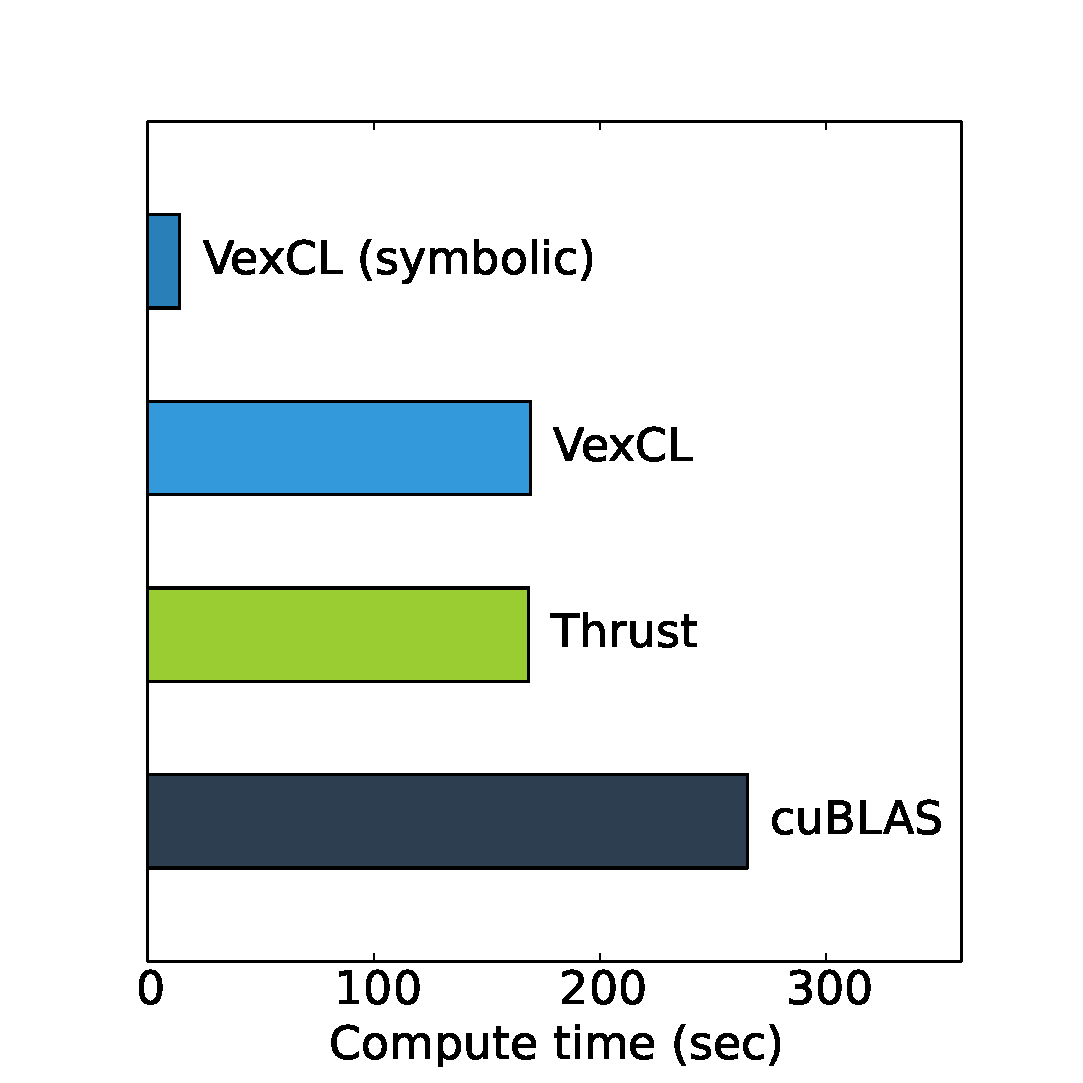
\includegraphics[width=\textwidth]{perfplot}
            \end{center}
        \end{column}
    \end{columns}
\end{frame}

\note{}

%----------------------------------------------------------------------------
\section{Оценка производительности}
\begin{frame}
    \sectionpage
\end{frame}

\note{}

%----------------------------------------------------------------------------
\begin{frame}[fragile]{Параметрическое исследование системы Лоренца}
    \begin{columns}
        \begin{column}{0.6\textwidth}
            \begin{block}{Система Лоренца}
                \vspace{-1\baselineskip}
                \begin{align*}
                    \dot{x} &= -\sigma \left( x - y \right), \\
                    \dot{y} &= R x - y - xz, \\
                    \dot{z} &= -bz + xy.
                    \label{eq:lorenz}
                \end{align*}
            \end{block}
            \begin{itemize}
                \item Будем одновременно решать большое число систем Лоренца
                    для различных значений $R$.
                \item Будем использовать библиотеку Boost.odeint.
            \end{itemize}
        \end{column}
        \begin{column}{0.4\textwidth}
            \begin{figure}
                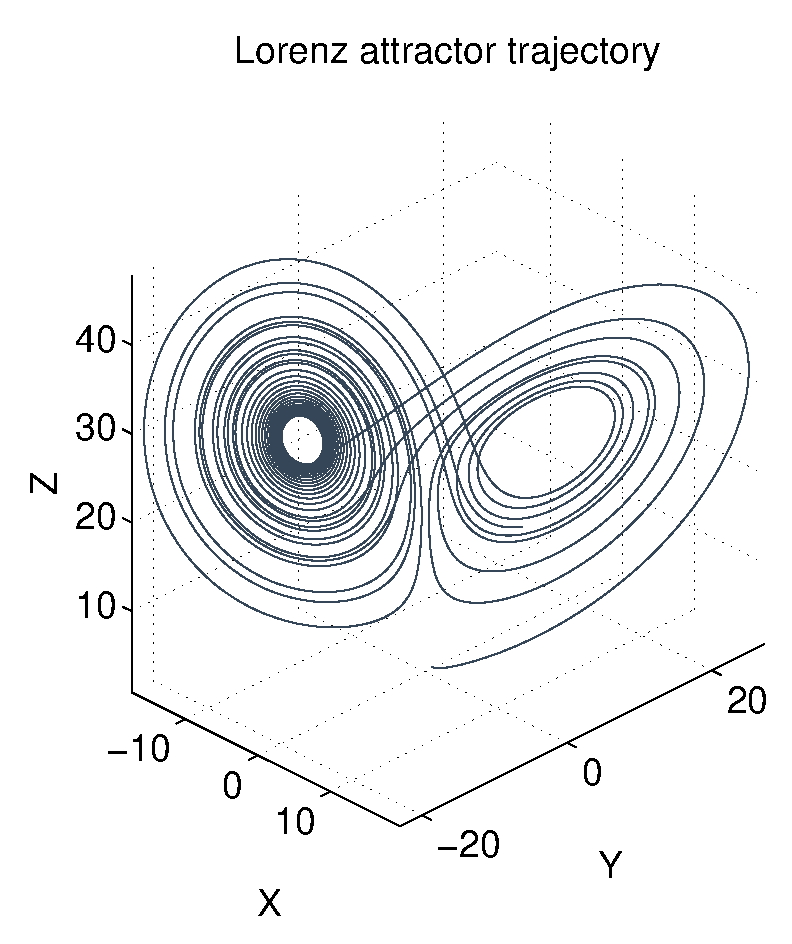
\includegraphics[width=\textwidth]{lorenz}
                \caption{Траектория аттрактора Лоренца}
            \end{figure}
        \end{column}
    \end{columns}
\end{frame}

\note[itemize]{
\item As an example, lets solve a Lorenz attractor system of ordinary
    differential equations.
\item Lorenz attractor is a particle that moves according to these governing
    equations. The plot on the right shows an example of particle trajectory in
    time.
\item We will solve large number of these Lorenz systems at once.  Each of the
    systems will have its own value for parameter R. That's why this is called
    a parameter study.
}

%----------------------------------------------------------------------------
\begin{frame}[fragile]{Вариант с использованием CUBLAS}
    \begin{itemize}
        \item CUBLAS~--- оптимизированная библиотека линейной алгебры от NVIDIA.
        \item Линейные комбинации (используемые в алгоритмах odeint):
            \begin{equation*}
                x_0 = \alpha_1 x_1 + \alpha_2 x_2 + \cdots + \alpha_n x_n
            \end{equation*}
            реализованы следующим образом:
    \end{itemize}
    \begin{exampleblock}{}
        \begin{lstlisting}[numbers=none,texcl=true]
cublasDset(...);        // $x_0 = 0$
cublasDaxpy(...);       // $x_0 = x_0 + \alpha_1 * x_1$
...
cublasDaxpy(...);       // $x_0 = x_0 + \alpha_n * x_n$
        \end{lstlisting}
    \end{exampleblock}
\end{frame}

\note{ }

%----------------------------------------------------------------------------
\begin{frame}[fragile]{Вариант с использованием Thrust}
    \begin{itemize}
        \item Thrust позволяет получить монолитное ядро:
    \end{itemize}
    \begin{columns}
        \begin{column}{0.70\textwidth}
            \begin{exampleblock}{Thrust}
                \begin{adjustbox}{width=0.95\textwidth,height=0.6\textheight,keepaspectratio}
                    \begin{lstlisting}
struct scale_sum2 {
    const double a1, a2;
    scale_sum2(double a1, double a2) : a1(a1), a2(a2) { }
    template<class Tuple>
    __host__ __device__ void operator()(Tuple t) const {
        thrust::get<0>(t) = a1 * thrust::get<1>(t) + a2 * thrust::get<2>(t);
    }
};

thrust::for_each(
        thrust::make_zip_iterator(
            thrust::make_tuple( x0.begin(), x1.begin(), x2.begin() )
            ),
        thrust::make_zip_iterator(
            thrust::make_tuple( x0.end(), x1.end(), x2.end() )
            ),
        scale_sum2(a1, a2)
        );
                    \end{lstlisting}
                \end{adjustbox}
            \end{exampleblock}
        \end{column}
        \begin{column}<2>{0.22\textwidth}
            \begin{exampleblock}{VexCL}
                \begin{adjustbox}{width=0.95\textwidth,height=0.6\textheight,keepaspectratio}
                    \begin{lstlisting}
x0 = a1 * x1 + a2 * x2;
                    \end{lstlisting}
                \end{adjustbox}
            \end{exampleblock}
        \end{column}
    \end{columns}
\end{frame}

\note{ }

%----------------------------------------------------------------------------
\begin{frame}[fragile]{Использование символьных переменных}
    \begin{itemize}
        \item Любые арифметические операции с экземплярами класса
            \code{vex::symbolic<>} выводятся в текстовый поток:
            \vspace{-0.5\baselineskip}
    \end{itemize}
    \begin{columns}
        \begin{column}{0.45\textwidth}
            \begin{exampleblock}{}
                \begin{lstlisting}
vex::generator::set_recorder( std::cout );
vex::symbolic<double> x, y = 6;
x = sin(y * 7);
                \end{lstlisting}
            \end{exampleblock}
        \end{column}
        \begin{column}{0.45\textwidth}
            \begin{exampleblock}{}
                \begin{verbatim}
double var1;
double var2 = 6;
var1 = sin( var2 * 7 );
                \end{verbatim}
            \end{exampleblock}
        \end{column}
    \end{columns}
    \vspace{\baselineskip}
    \begin{itemize}
        \item Мы можем подать символьные переменные на вход шаблонной функции и
            получить запись алгоритма в виде кода \CC.
            \begin{itemize}
                \item Используем один шаг алгоритма Рунге-Кутты из Boost.odeint
                    для получения монолитного ядра.
            \end{itemize}
    \end{itemize}
\end{frame}

\note{}

\end{document}
